\documentclass[../main.tex]{subfiles}
\begin{comment}
\addbibresource{../bib/bibliography.bib} 
\end{comment}
\begin{document}

\subsection{Result}
\begin{figure}[h]
    \centering
    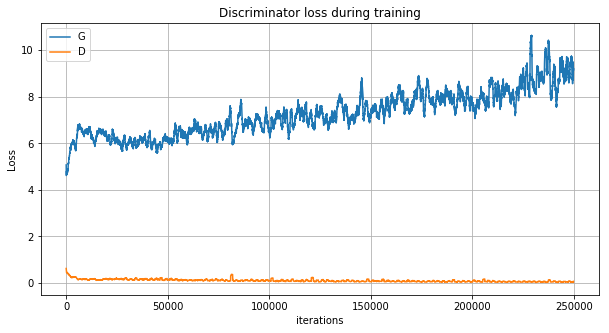
\includegraphics[width=\textwidth]{both_loss.png}
    \caption{The loss of the generator and discriminator during training}
    \label{fig:both_loss}
\end{figure}
\begin{figure}[h]
    \centering
    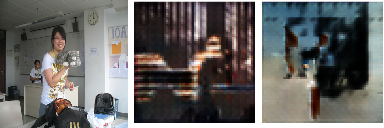
\includegraphics[width=\textwidth]{merge_girl.png}
    \caption{Caption: \textit{Girl holding cat stuffed animal.} \\From left to right; Captioned Image, Output after 50 epochs, Output after 100 epochs}
    \label{fig:res_girl}
\end{figure}
\begin{figure}[h]
    \centering
    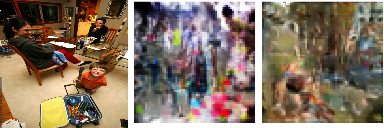
\includegraphics[width=\textwidth]{merge_suit.png}
    \caption{Caption: \textit{A little boy shows off his suitcase full of toys.} \\From left to right; Captioned Image, Output after 50 epocs, Output after 100 epochs}
    \label{fig:res_suit}
\end{figure}
\begin{figure}[h]
    \centering
    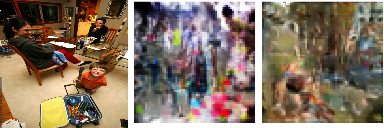
\includegraphics[width=\textwidth]{merge_jack.png}
    \caption{Caption: \textit{A man with a jackhammer demolishing cement.} \\
    From left to right; Captioned Image, Output after 50 epochs, Output after 100 epochs}
    \label{fig:res_jack}
\end{figure}

In Figure \ref{fig:both_loss} the result of the loss function can be seen for the Discriminator $D$ and Generator $G$. The plot is the result of a moving average with a window size of 1000 data points to identify the trend of the loss function. Looking specifically at the discriminator loss we see that the loss seem to converge towards 0 which means the generator isn't able to deliver good enough images. There is an apparent negative correlation between the Generator and Discriminator loss which it should be since they are playing a min-max game, though, the generator shouldn't be losing this bad. We believe that is because of the complex captions in \texttt{flickr\_30k} dataset. We might have had better success to use dataset with less classes, such as \texttt{Oxford 102 Flowers} or the like. Datasets which handles far less object classes in their captions. Unfortunately there was no time to train such a network when we realised that.
We see in Figure \ref{fig:res_girl}, \ref{fig:res_jack}, \ref{fig:res_suit} that even after 100 epochs the scene depicted in the generataed image is not apparent.
\begin{figure}[h]
    \centering
    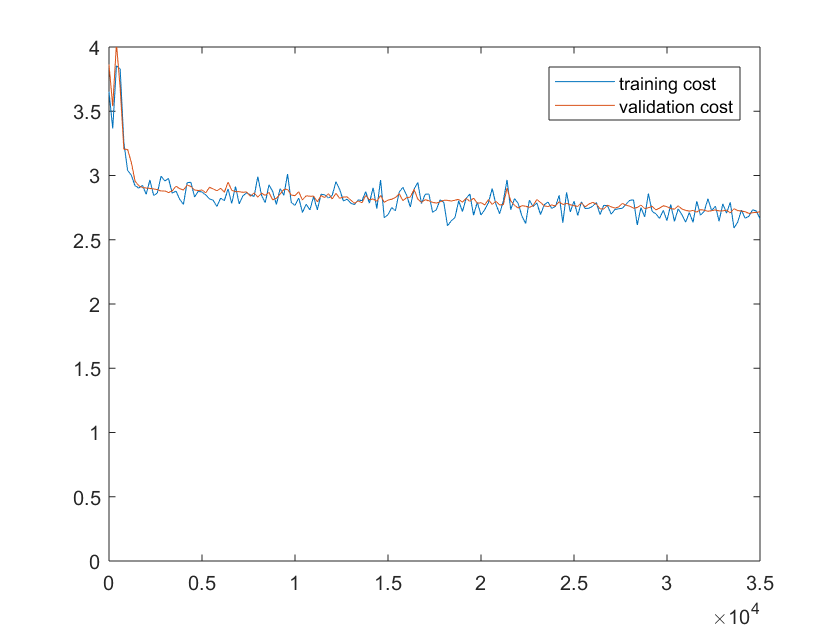
\includegraphics[width=0.5\textwidth]{1.png}
    \caption{Training and validation set loss every 200th update.}
    \label{fig:speechloss}
\end{figure}

In Figure \ref{fig:speechloss} we can see how the validation and training cost is converging towards ~2.5. The best test set accuracy achieved with the Speech Command dataset on 8-layer network was 12.31 \%. The table 2 below displays the top results achieved with this network. Different number of layers with different amount of hidden nodes were tested but the top results were achieved with 8-layer network where the nodes settings were: 100,100,100,100,70,50,50,30.

\begin{center}
 \begin{tabular}{|c c c c c c c|} 
 \hline
 $\eta_{min}$ & $\eta_{max}$ & $ns$  & $l$ & $\lambda$ & $nbatch$ & accuracy\\ [0.5ex] 
 \hline\hline
 1e-3 & 1e-1 & 6*110 & 5 & 0.0001 & 100 & 12.31 \\ 
 \hline
 1e-3 & 1e-1 & 5*110 & 5 & 0.0001 & 100 & 11.94 \\
 \hline
 1e-3 & 1e-1 & 6*110 & 3 & 0.001 & 100 & 11.30 \\[1ex]
\hline
\end{tabular}
\caption{Table 2}
\end{center}

\subsection{Future Work}
Time limitation: Since there is no enough time to training audio2text, we could not covering all words. Thus, we just training limit number of word and assume that audio2text is done. With more time on hands we would also consider trying out implementing Convolutional Neural Network for speech recognition with the Speech Command dataset. We would also try to preprocess the speech data differently using more amount of mffcs and see whether that affects how well the network learns to label the audio files.
\par
The above image generation in pixel level based on GAN is currently focused on the generation of a single object. When we want to generate complex scenes with multiple interactive objects in the image based on the text, it is very difficult to understand this high-level semantic information from the pixel level.

Extensions of this work include using the condition augmentation presented in \cite{zhang2017stackgan++} instead of the perturbation approach. Another extension would be to actually use the scene information that lies in the ordering of the words instead of just taking the minimum and maximum elements and thus ignoring the order. Another improvement to our approach is to stack discriminators and generators on top of each other \cite{zhang2017stackgan++} which could yield in improved quality and thus the creation of more realistic images. 
\end{document}